\section{Maximum Flow}
\subsection{Flow networks}
\label{sub:flow_networks}

\begin{description}
\descitem{26.1-1} \textit{Show that splitting an edge in a flow network yields an equivalent network. More formally, suppose that flow network $G$ contains edge $(u,v)$ and we create a new flow network $G'$ by creating a new vertex $x$ and replacing $(u,v)$ by new edges $(u,x)$ and $(x,v)$ with $c(u,x) = c(x,v) = c(u,v)$. Show that a maximum flow in $G'$ has the same value as a maximum flow in $G$.}

\begin{ex}
  Soit un réseau de flot $G$, une arête $(u,v)$ et $f_G$ un flot associé. Par construction de $G'$ et conservation d'un flot, on a $f_G(u,v) = f_{G'}(u,x) = f_{G'}(x,v)$, donc $|f_G| = |f_{G'}|$.

  Réciproquement, soit un réseau $G'$ obtenu par une division d'arête en $(u,x)$ et $(x,v)$. Comme il n'y a qu'un flot entrant et sortant en $x$, on a toujours par conservation $f_{G'}(u,x) = f_{G'}(x,v)$. Sachant que $c(u,x) = c(x,v)$, on peut fusionner les arêtes $(u,x)$ et $(x,v)$ tout en laissant $|f_{G'}|$ inchangée.
  
Plus généralement, dans un réseau $G$ ayant un sommet $x$ tel que $d^+(x) = d^-(x) = 1$, en posant $c(u,v) = \min(c(u,x),c(u,v))$ on peut fusionner les arêtes $(u,x)$ et $(x,v)$ tout en laissant $|f_{G}|$ inchangée (cf. fig. \ref{fig:edge-fusion}).

\begin{figure}[H]
\centering

\begin{subfigure}[t]{.45\textwidth}
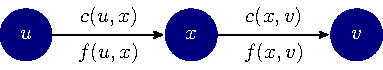
\includegraphics{img/26_1-1/26_1-1_1.pdf}
\end{subfigure}
~
\begin{subfigure}[t]{.45\textwidth}
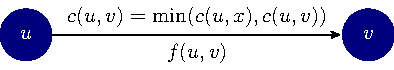
\includegraphics{img/26_1-1/26_1-1_2.pdf}
\end{subfigure}
\caption{Fusionnement d'arête}
\label{fig:edge-fusion}
\end{figure}

Ceci est valide sur un chemin dans lequel tous les sommets intermédiaires $x$ vérifient $d^+(x) = d^-(x) = 1$ (cf. fig. \ref{fig:edge-fusion-2}).


\begin{figure}[H]
\centering
  \begin{subfigure}[t]{\textwidth}
    \centering
    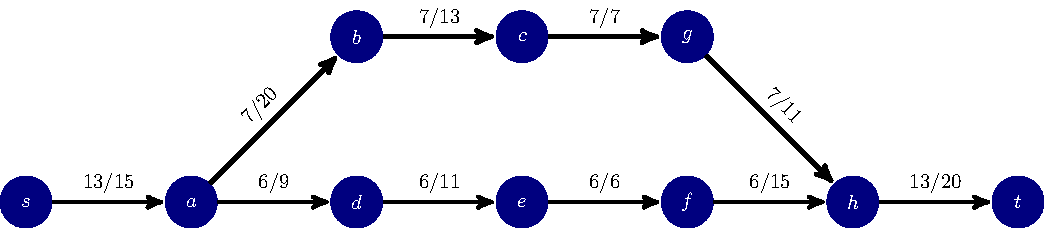
\includegraphics{img/26_1-1/26_1-1_3.pdf}
    \caption{Un réseau $G'$ pouvant être réduit à un réseau équivalent $G$, dans le sens où leur flot maximal sont égaux.}
  \end{subfigure}

  \begin{subfigure}[t]{\textwidth}
    \centering
    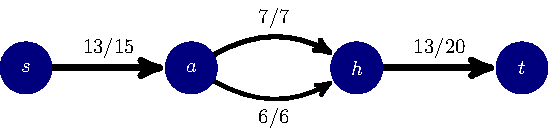
\includegraphics{img/26_1-1/26_1-1_4.pdf}
    \caption{Fusion du chemin $(a,b,c,g,h)$  et du chemin $(a,d,e,f,h)$ en $(a,h)$.}
  \end{subfigure}

  \begin{subfigure}[t]{0.49\textwidth}
    \centering
    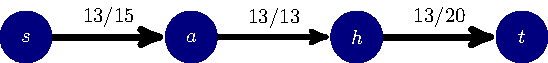
\includegraphics{img/26_1-1/26_1-1_5.pdf}
    \caption{Fusion des deux arêtes $(a,h)$.}
  \end{subfigure}
~
  \begin{subfigure}[t]{0.49\textwidth}
    \centering
    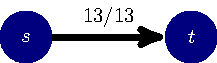
\includegraphics{img/26_1-1/26_1-1_6.pdf}
    \caption{Le réseau $G$ final.}
  \end{subfigure}
  \caption{Fusionnement de chemin unidirectionnel}
  \label{fig:edge-fusion-2}
\end{figure}
\end{ex}

\descitem{26.1-2} \textit{}
\descitem{26.1-3} \textit{}
\descitem{26.1-4} \textit{}
\descitem{26.1-5} \textit{}
\descitem{26.1-6} \textit{}
\descitem{26.1-7} \textit{}

\end{description}
